\subsection{Component Identification in Figure T-1}
\label{T6C02}

\begin{figure}[th]
    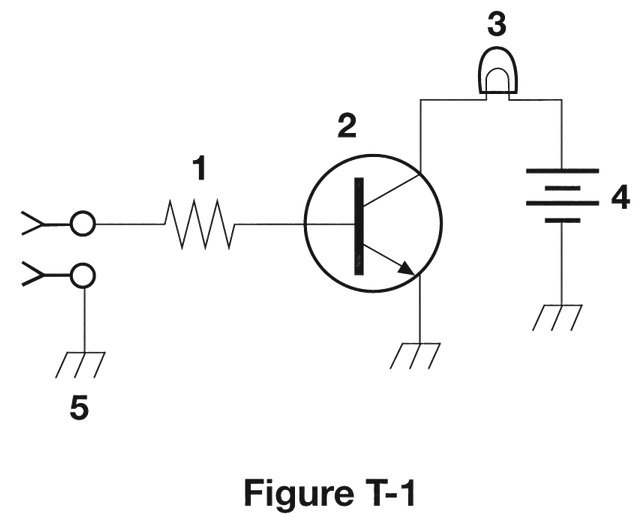
\includegraphics[width=0.5\textwidth]{tech/images/t1.png} 
\end{figure}

\begin{tcolorbox}[colback=gray!10!white,colframe=black!75!black,title=T6C02]

What is component 1 in figure T-1?
\begin{enumerate}[label=\Alph*)]
    \item \textbf{Resistor}
    \item Transistor
    \item Battery
    \item Connector
\end{enumerate}
\end{tcolorbox}

\subsubsection{Intuitive Explanation}
Imagine you’re building a simple circuit, like a tiny flashlight. You have a battery to power it, wires to connect everything, and a light bulb to shine. But wait! If you connect the battery directly to the bulb, it might burn out because too much electricity flows through it. That’s where a resistor comes in—it’s like a speed bump for electricity. It slows down the flow so your bulb doesn’t get fried. In this question, component 1 is that helpful speed bump, also known as a resistor.

\subsubsection{Advanced Explanation}
In electrical circuits, a resistor is a passive two-terminal component that implements electrical resistance as a circuit element. Resistors are used to reduce current flow, adjust signal levels, divide voltages, and bias active elements. The resistance \( R \) of a resistor is given by Ohm's Law:

\[
V = IR
\]

where \( V \) is the voltage across the resistor, \( I \) is the current through the resistor, and \( R \) is the resistance. In the context of the question, component 1 is identified as a resistor based on its symbol and function in the circuit diagram (Figure T-1). Resistors are typically represented by a zigzag line in circuit diagrams, distinguishing them from other components like transistors, batteries, and connectors.

% Prompt for generating the diagram: Include a circuit diagram labeled Figure T-1 with a resistor clearly marked as component 1.